\section{Implemented changes}\label{jiveImpl}%hva ble gjort, hvordan bruke funksjonene. Ikke så mye om hvordan. begrunne prioriteter?
~\\

%identifisering av instansierte grensesnitt, lambdaer og abstrakte klaser
The first change to be implemented was the identification and presentation of instantiated interfaces, which are now displayed in the diagrams with an appropriate icon, as well as being labeled with the interface it implements, instead of the generic class name that it is assigned by default.
An example of this is shown in \autoref{fig:JiveNewIcon}
This function was also expanded to identify and label instances of abstract classes, and the lambda-expressions that were introduced with Java 8.
In order to still allow the actual class name to be visible, the tool-tip shown when hovering the mouse pointer over an object remains unmodified, showing the actual class name and icon.
\begin{figure}[H]
	\centering
	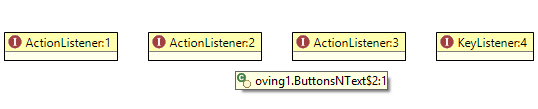
\includegraphics[width=\textwidth]{UIJiveInterfaceIcon}
	\caption[A view of how instantiated interfaces are shown after the modification.]{A view of how instantiated interfaces are shown after the modification. Also shown, is the tool-tip text for the second instance from the left. Originally, they would be labeled as 'ButtonsNText\$1:1', 'ButtonsNText\$2:1' and so on, with the green class-icon.}
	\label{fig:JiveNewIcon}
\end{figure}
~\\

%utvidelse av filteret
The filtering function was expanded with the ability to specify packages that are not to be excluded from the execution model, as suggested in \autoref{jiveSuggestions}.
Adding a package to be included is as simple as adding a `+' in front of the package-name when adding it to the filter.
As an example, the default filter excludes the javax package, and any subpackages that are not specifically listed with a `+' in front.
When adding the line `+javax.swing.*' in order to let swing components through the filter, one will let every subpackage of 'javax.swing' though the filter as well, which is the intended design.
Unfortunately, there are a lot of classes in both swing, and its subpackages that are not used directly when writing swing-programs, and that a user will have no interest in seeing in the diagrams.
This can result in very poor performance, as unnecessary events are logged, and cluttered diagrams, but can be handled by adding the unwanted classes to the filter for exclusion.
Depending on the package in question, the amount of extra items added to the filter can become quite large, and identifying all unwanted classes and subpackages may take hours at worst.
One weakness in the filter, related to the problem of unwanted packages, is that due to its design, allowing the contents of a package, will also allow any classes that are contained directly within the parent package, as this also has to be removed from the internal list of exclusions that make up the filter.
This is not a big problem in the case of `javax.swing', as the `javax' package does not contain any classes, but there are definitely other packages that will show this behavior.
~\\

With an appropriate filter, one will get to see the connection between listeners and the objects they listen to, via the existing object-containment-links, given that the listener-field is actually visible.
An unfortunate behavior of JIVE is that only the fields defined within a class are visible in figures of instances of that class.
Any inherited fields are not shown, and this is unfortunately the case for many UI-components in the swing-framework.
The quick solution to this problem, simply showing all inherited fields, would result in a large amount of useless information, cluttering the diagram, and hiding the useful information.
In lack of a good solution, and with a desire to not make large fundamental changes, preferring minor adjustments that use the existing framework in better ways.
Assuming that the listener-field is visible, this would in most cases be a list of listeners, and so the filter would also need to allow that type of list through.
As there are a large amount of lists in use behind the scenes in a graphical program, this would be another source of unnecessary clutter.
The filter itself is likely to become very large due to the extra exclusions needed to hide unwanted classes, as a consequence of letting something through.
~\\

There is currently no easy way to quickly swap the entire filter for another one, but the filters are stored in eclipses launch configuration files.
These configurations are stored as XML-files, and can be easily modified in any text editor.
By managing these files directly, a user can quickly swap the entire filter, copy it to another launch-configuration file, or share it with others.
After modifying these files, Eclipse requires a restart to detect the changes, adding to the time and effort required to make any changes this way.
This is of course not a good way of handling the issue, and ways of improving this should be explored in the future.
~\\

%isolert visning av sekvens
The isolated view was implemented as a separate view-tab, and does what was proposed in \autoref{fig:seqOving4IsolatedMock}: it displays the events caused by the selected event, and hides everything else.
\autoref{fig:MMI-oving4-SeqIsoDiag-AWT-Event-Thread} shows what \autoref{fig:seqOving4IsolatedMock} ended up looking like after the modification.
\autoref{fig:MMI-oving4-SeqIsoDiag-valueChanged} shows a similar, but slightly more complex situation in the isolated view.
By right clicking on an event in the regular sequence diagram, and selecting the `Isolated view' option, shown in \autoref{fig:UISeqRightClickNew},  the isolated view is triggered.
It is also possible to further focus on a part of the diagram from within the isolated view, by right clicking on the desired event, and selecting the `Isolated view' option again.
All of the functionality from the regular sequence diagram has been retained in the isolated view, so that the only difference is what parts of the execution are visible.
\begin{figure}[H]
	\centering
	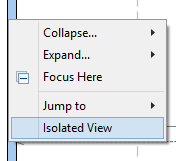
\includegraphics{UIseqRightClickNew}
	\caption{The new 'Isolated view' option.}
	\label{fig:UISeqRightClickNew}
\end{figure}
~\\
\begin{figure}[H]
	\centering
	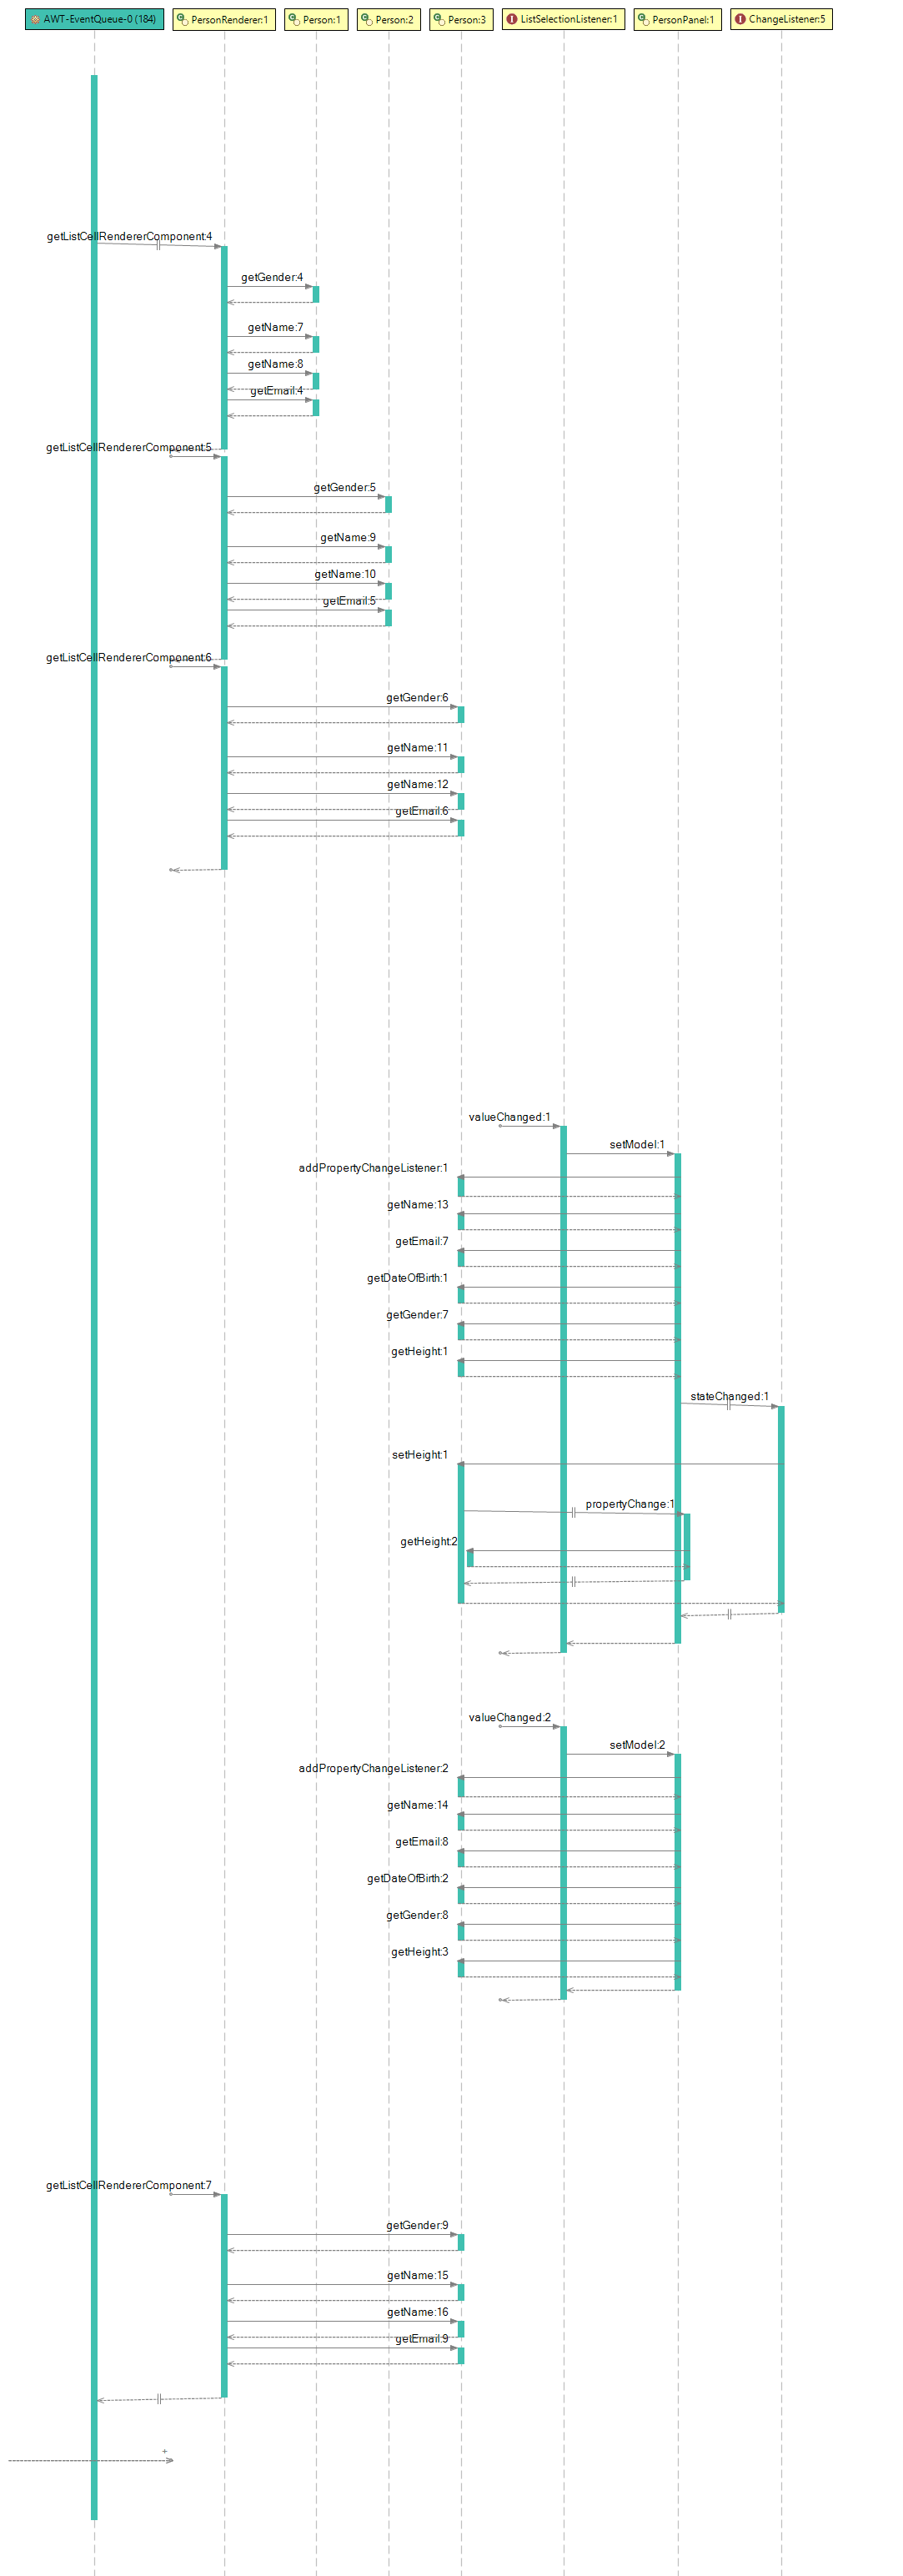
\includegraphics[width=\textwidth, trim= 0cm 50cm 0cm 0cm, clip]{MMI-oving4-SeqIsoDiag-AWT-Event-Thread}
	\caption[How \autoref{fig:seqOving4CrossLines} looks in the isolated view.]{How \autoref{fig:seqOving4CrossLines} looks in the isolated view. The three last elements shown on the top are referred to in parts of the diagram not shown. This view was achieved by selecting the 'AWT-EventQueue' lifeline for the isolated view.}
	\label{fig:MMI-oving4-SeqIsoDiag-AWT-Event-Thread}
\end{figure}
~\\
\begin{figure}[H]
	\centering
	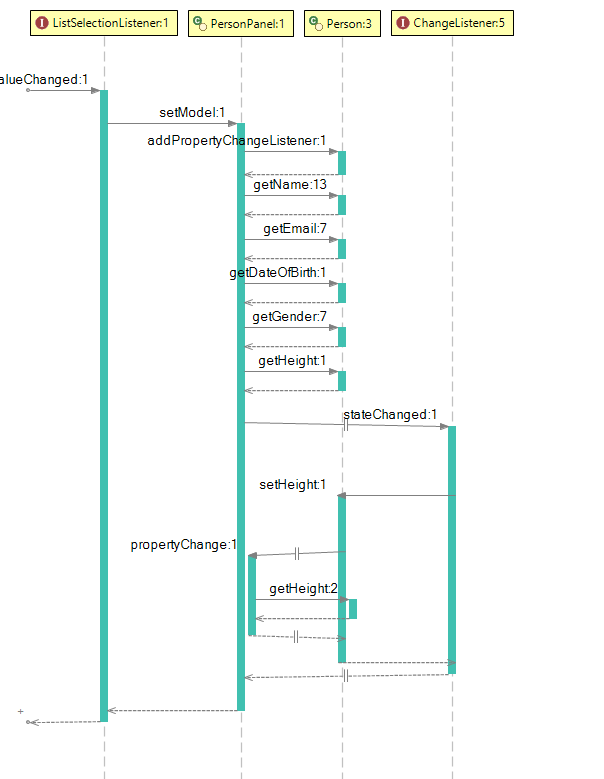
\includegraphics[width=\textwidth, trim= 0cm 0cm 0cm 0cm, clip]{MMI-oving4-SeqIsoDiag-valueChanged}
	\caption{Another example  of the isolated view, showing a significantly reorganized diagram.}
	\label{fig:MMI-oving4-SeqIsoDiag-valueChanged}
\end{figure}
 ~\\

%mer avslappede søkekrav - er ikke utført for alle typer søk, er det verd å nevne i det hele tatt?
The searching functionality was relaxed by allowing partial matches, and disabling case sensitivity.
While relaxing the search may cause false positives, a user should be able to identify such cases quickly, or at least identify the results they were looking for.
The fact that partial matches and case insensitivity is the standard behavior in most search-engines, sets an expectation for the behavior of the search within JIVE.
Unfortunately, due to the existing implementation consisting of separate searching- and matching-methods for each search type, not all searches were updated to this relaxed state.

%hvorfor ble ikke alle forslag impementert? - tid for å bli kjent med jive, eclipse-plugins
